%! Author = sriadityavedantam
%! Date = 4/8/26

\section{Normal Varieties}

\subsection{Integrally Normal}

Let
\[
    A = \c[x,y]/(y^2 - x^2 - x^3).
\]
We claim that $A$ is not integrally closed.
Recall that if $K = \Frac(A)$, then
\[
    t \coloneqq \frac{y}{x}\in K.
\]
Then
\[
    t^2 = \frac{y^2}{x^2} = \frac{x^2 + x^3}{x^2} = 1 + x \in A.
\]
Thus
\[
    t^2 - 1 - x = 0,
\]
which is a monic polynomial equation over $A$ satisfied by $t$.
Hence $t$ is integral over $A$.
But $t \notin A$.
Therefore $A$ is not integrally closed.
If $p/q \in \c(X)$, assume that $p/q$ is integral over $\c[X]$.
Then there exists a monic equation
\[
    \left(\frac{p}{q}\right)^n + a_1\left(\frac{p}{q}\right)^{n-1} + \cdots + a_n = 0
\]
with $a_i \in \c[X]$.
Multiplying through by $q^n$, we get
\[
    p^n + a_1 p^{n-1}q + \cdots + a_n q^n = 0.
\]
Hence
\[
    p^n = -\left(a_1 p^{n-1}q + \cdots + a_n q^n\right).
\]
So $q$ divides $p^n$ in $\c[X]$.
If $\c[X]$ is integrally closed, this forces $p/q \in \c[X]$.

\begin{definition}[Normal]
    An irreducible affine variety $X$ is normal if and only if $\c[X]$ is integrally closed.
\end{definition}

Generally, an irreducible quasi-projective variety $X$ is normal if and only if every point has a normal affine neighborhood.

\begin{lemma*}{
    If $X$ is an irreducible quasi-projective variety, then $X$ is normal if and only if $\o_x$ is integrally closed for all $x\in X$.
}
\end{lemma*}

\begin{lemma}{
    $X$ is normal if and only if every finite birational morphism to $X$ is an isomorphism.
}
\end{lemma}

\begin{theorem*}{
    An irreducible curve is normal if and only if it is smooth.
}
\end{theorem*}

\begin{theorem*}{
    If $X$ is an irreducible quasi-projective variety and is smooth, then it is normal.
}
\end{theorem*}

\begin{theorem*}{
    If $X$ is an irreducible quasi-projective variety and is normal, then the set of singular points in $X$ has codimension at least $2$.
}
\end{theorem*}

\[
    \{x^2 + y^2 = z^2\} \eqqcolon S \subseteq \c^3.
\]

\begin{figure}[H]
    \centering
    \tikzset{every picture/.style={line width=0.75pt}}
    \colorbox{white}{%
        \color{black}
        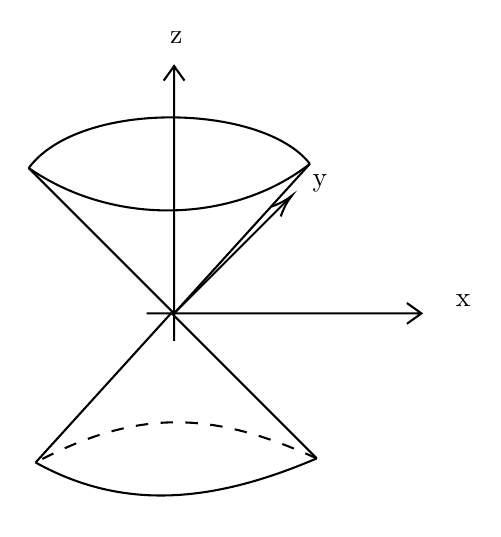
\begin{tikzpicture}[
            x=0.75pt,
            y=0.75pt,
            yscale=-1,
            xscale=1,
            every node/.style={text=black},
            every path/.style={draw=black},
            line width=0.75pt
        ]
            \draw  (267.21,138.16) -- (399.61,138.16)(280.45,19) -- (280.45,151.4) (392.61,133.16) -- (399.61,138.16) -- (392.61,143.16) (275.45,26) -- (280.45,19) -- (285.45,26);
            \draw    (280.45,138.16) -- (335.81,82.8);
            \draw [shift={(337.23,81.38)}, rotate = 135] [color={rgb,255:red,0;green,0;blue,0}][line width=0.75] (10.93,-3.29) .. controls (6.95,-1.4) and (3.31,-0.3) .. (0,0) .. controls (3.31,0.3) and (6.95,1.4) .. (10.93,3.29);
            \draw    (280.45,138.16) -- (210.4,68.11);
            \draw    (345.86,66.12) -- (280.45,138.16);
            \draw    (210.4,68.11) .. controls (251.61,96.65) and (309.35,94.66) .. (345.86,66.12);
            \draw    (210.4,68.11) .. controls (235.02,34.93) and (323.29,36.92) .. (345.86,66.12);
            \draw    (279.12,137.96) -- (349.17,208.01);
            \draw    (213.72,210) -- (279.12,137.96);
            \draw    (349.17,208.01) .. controls (295.5,231) and (253.5,232) .. (213.72,210);
            \draw  [dash pattern={on 4.5pt off 4.5pt}]  (349.17,208.01) .. controls (326.88,197.93) and (307.24,191.83) .. (287.62,190.79) .. controls (264.41,189.55) and (241.24,195.37) .. (213.72,210);

            \draw (345.66,69.9) node [anchor=north west][inner sep=0.75pt]   [align=left] {y};
            \draw (414.69,127.64) node [anchor=north west][inner sep=0.75pt]   [align=left] {x};
            \draw (277,1) node [anchor=north west][inner sep=0.75pt]   [align=left] {z};
        \end{tikzpicture}
    }
\end{figure}

We claim that $S$ is normal.

\begin{example}{
    Let
    \[
        S = \{x^2 + y^2 = z^2\}\subseteq \c^3.
    \]
    Then $S$ is normal.
}
    With $u,v\in \c(x,y)$, every element of $\c(S)$ has the form $u + vz$.
    If $\alpha = u + vz \in \c(S)$ is integral over $\c[S]$, then it is also integral over $\c[x,y]$ since $\c[S]$ is finite over $\c[x,y]$.

    The conjugate of $\alpha$ over $\c(x,y)$ is $u-vz$.
    So the minimal polynomial of $\alpha$ over $\c(x,y)$ is
    \[
        T^2 - 2uT + u^2 - (x^2+y^2)v^2.
    \]
    If $\alpha$ is integral over $\c[x,y]$, then the coefficients of this polynomial are integral over $\c[x,y]$.
    Since $\c[x,y]$ is integrally closed, it follows that
    \[
        2u \in \c[x,y],
    \]
    hence
    \[
        u\in \c[x,y].
    \]
    Also
    \[
        u^2 - (x^2+y^2)v^2 \in \c[x,y].
    \]
    Since
    \[
        x^2+y^2 = (x+iy)(x-iy),
    \]
    and these factors are irreducible and coprime in $\c[x,y]$, it follows that $v\in \c[x,y]$.
    Therefore $\alpha\in \c[S]$.
    So $\c[S]$ is integrally closed, and hence $S$ is normal.
\end{example}

\subsection{Normalization}

\begin{figure}[H]
    \centering
    \tikzset{every picture/.style={line width=0.75pt}}
    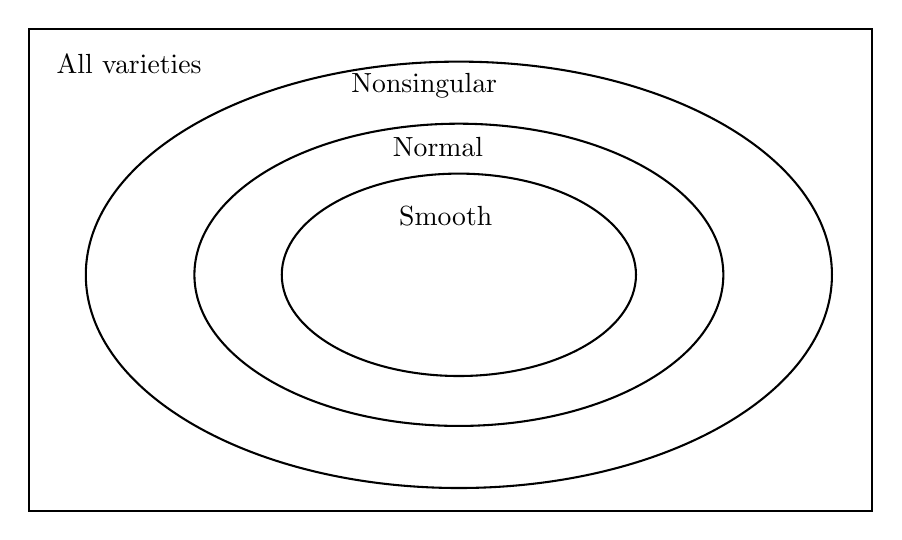
\begin{tikzpicture}[x=0.75pt,y=0.75pt,yscale=-1,xscale=1]
        \draw   (195.5,138.57) .. controls (195.5,81.84) and (275.98,35.86) .. (375.25,35.86) .. controls (474.52,35.86) and (555,81.84) .. (555,138.57) .. controls (555,195.3) and (474.52,241.29) .. (375.25,241.29) .. controls (275.98,241.29) and (195.5,195.3) .. (195.5,138.57) -- cycle ;
        \draw   (247.83,138.57) .. controls (247.83,98.36) and (304.88,65.76) .. (375.25,65.76) .. controls (445.62,65.76) and (502.67,98.36) .. (502.67,138.57) .. controls (502.67,178.78) and (445.62,211.38) .. (375.25,211.38) .. controls (304.88,211.38) and (247.83,178.78) .. (247.83,138.57) -- cycle ;
        \draw   (289.92,138.57) .. controls (289.92,111.64) and (328.12,89.81) .. (375.25,89.81) .. controls (422.38,89.81) and (460.58,111.64) .. (460.58,138.57) .. controls (460.58,165.5) and (422.38,187.33) .. (375.25,187.33) .. controls (328.12,187.33) and (289.92,165.5) .. (289.92,138.57) -- cycle ;
        \draw   (168,20) -- (574.5,20) -- (574.5,252.29) -- (168,252.29) -- cycle ;

        \draw (180,31) node [anchor=north west][inner sep=0.75pt]   [align=left] {All varieties};
        \draw (322,40) node [anchor=north west][inner sep=0.75pt]   [align=left] {Nonsingular};
        \draw (342,71) node [anchor=north west][inner sep=0.75pt]   [align=left] {Normal};
        \draw (345,104) node [anchor=north west][inner sep=0.75pt]   [align=left] {Smooth};
    \end{tikzpicture}
    \caption{From Mumford's \textit{Red Book of Varieties and Schemes}.}
\end{figure}

\begin{proposition*}{
    Let $Y = \spec(S)$ be normal.
    Let $R\subset S$ be a finitely generated subring such that $S$ is finite over $R$.
    Then $X \coloneqq \spec(R)$ need not be normal.
}
\end{proposition*}

Let $S = \c[x,y]$, so $\spec S = \aa^2$.
Take
\[
    R = \c + I,
\]
where $I$ is the ideal of the two points $(0,0)$ and $(1,0)$.
Then
\[
    0\to R\to S\to S/R\to 0,
\]
and
\[
    S/R \cong \c\oplus \c.
\]

\begin{definition}[Normalization]
    Let $X$ be an irreducible quasi-projective variety.
    A normalization of $X$ is a normal irreducible variety denoted by $X^\nu$ together with a morphism
    \[
        \pi : X^\nu\to X
    \]
    which is finite and birational.
    If $X$ is not irreducible, then write $X = \bigcup X_i$ as the union of irreducible components and define
    \[
        X^\nu = \bigsqcup X_i^\nu.
    \]
\end{definition}

\begin{theorem*}[Geometric Noether Normalization Theorem]{
    Let $X$ be an affine variety of dimension $n$.
    Then there exists a finite morphism
    \[
        \pi \colon X \to \aa^{n}
    \]
}
\end{theorem*}

\begin{definition}[$V(S)$]
For every subset $S\subset R$, we have
\begin{align*}
V(S) &= \{x\in\spec(R) : f(x) = 0 \text{ for all } f\in S\} \\
&= \{\mathfrak{p} : \mathfrak{p} \text{ is a prime ideal and } \mathfrak{p}\supseteq S\}.
\end{align*}
\end{definition}

\begin{theorem}{
Let $R$ be an integral domain finitely generated over $\c$, and let $P\subset R$ be a prime ideal.
Then
\[
\dim(R/P) = \tdeg_{\c}\Frac(R/P).
\]
}
We can reduce this proof to the case $P = \sqrt{(f)}$, or geometrically, the case $Z = V((f))$.
Suppose we have the decomposition
\[
\sqrt{(f)} = P\cap P_1^{\prime}\cap\ldots\cap P_t^{\prime}
\]
in $R$.
If $Z_i^{\prime} = V(P_i^{\prime})$, then $Z,Z_1^{\prime},\ldots,Z_t^{\prime}$ are the components of $V((f))$.
Pick an affine open $U_0\subset X$ such that
\begin{align*}
U_0\cap Z &\neq \varnothing,\\
U_0\cap Z_i^{\prime} &= \varnothing,\qquad i = 1,\ldots,t.
\end{align*}
Let $U_0 = X_g$, where
\[
g\in P_1^{\prime}\cap\ldots\cap P_t^{\prime},\qquad g\notin P.
\]
Then replace $X$ by $U_0$, $R$ by $R_{(g)}$, and in the new setup
\begin{align*}
V_{U_0}((f)) &= V_X((f))\cap U_0 \\
&= Z\cap U_0
\end{align*}
is irreducible.
Hence in $R_{(g)}$, $\sqrt{(f)} = P\cdot R_{(g)}$ is prime.
We can now use Noether normalization to find a morphism
\[
X\overset{\pi}{\longrightarrow}\aa^n,
\]
equivalently
\[
R\overset{\pi^\ast}{\hookleftarrow} \c[x_1,\ldots,x_n] = S.
\]
Let $K$ be the quotient field of $R$ and let $L$ be the quotient field of $S$.
Then $K/L$ is a finite algebraic extension.
Let
\[
f_0 = N_{K/L}(f).
\]
Then we claim $f_0\in S$ and
\[
P\cap S = \sqrt{(f_0)}.
\]

If we prove this, the theorem follows.
For $R/P$ is an integral extension of $S/(S\cap P)$, so
\[
\tdeg_{\c} R/P = \tdeg_{\c} S/(S\cap P).
\]
But $S$ is a UFD, so if $S\cap P$ is height one, then it is principal.
Therefore $P\cap S = (f_{00})$ for some irreducible $f_{00}\in S$, and hence
\[
\tdeg_{\c} S/(S\cap P) = n-1.
\]

We check first that $f_0\in P\cap S$.
Let
\[
Y^n + a_{1}Y^{n-1} + \ldots + a_n = 0
\]
be the irreducible equation satisfied by $f$ over the field $L$.
Then $f_0$ is a power of $a_n$.
Moreover, all the $a_i$ are symmetric functions in the conjugates of $f$, therefore the $a_i$ are elements of $L$ integral over $S$.
Hence $a_i\in S$.
In particular $f_0\in S$, and since
\begin{align*}
    0 &= a_n^{m-1}(f^n + a_{1}f^{n-1} + \ldots + a_n) \\
    &= f(a_n^{m-1}f^{n-1} + a_n^{m-1}a_{1}f^{n-2} + \ldots + a_n^{m-1}a_{n-1}) + f_0,
    \end{align*}
we also have $f_0\in P$.
Finally suppose $g\in P\cap S$.
Then $g\in P$, hence $g^n = fh$ for some integer $n$ and some $h\in R$.
Taking norms, we find that
\begin{align*}
g^{n[K:L]} &= N_{K/L}(g^n) \\
&= N_{K/L}(f)N_{K/L}(h)\in (f_0),
\end{align*}
since $N_{K/L}(h)$ is an element of $S$ by the reasoning used before.
Therefore $g\in \sqrt{(f_0)}$, and so $P\cap S = \sqrt{(f_0)}$.
\end{theorem}

\begin{theorem}{
The normalization of any quasi-projective variety exists and is unique up to isomorphism compatible with $\pi$.
}
Assume $X$ is affine.
Let
\[
A \coloneqq \{f\in\c(X) : f \text{ is integral over } \c[X]\}.
\]
Then $A$ is a subring of $\c(X)$.
Thus there are no zero divisors in $A$, and it is finitely generated over $\c$ by Noether normalization.
Then $A$ is the ring of regular functions on an affine variety.
Let
\[
X^\nu \coloneqq \spec(A).
\]
We claim that $X^\nu$ is the normalization of $X$, with morphism
\[
X^\nu\overset{\varphi}{\longrightarrow} X
\]
induced by $\c[X]\hookrightarrow A$.
In order to prove this, we must check that $\varphi$ is birational and finite.
\end{theorem}

If we let
\[
X \coloneqq \spec\bigl(\c[x,y]/(y^2 - x^3)\bigr),
\]
then $\c[X]$ is not normal.